%-------------------------------------------------------------------------------
%	SECTION TITLE
%-------------------------------------------------------------------------------
\cvsection{Projects}


%-------------------------------------------------------------------------------
%	CONTENT
%-------------------------------------------------------------------------------
\begin{cventries}

    %---------------------------------------------------------
    \cventry
    {Personal project to celebrate the bachelor degree} % Project name
    {Model Rocket} % Institution
    {Personal Workshop, Como, Italy} % Location
    {Jul. 2023} % Date(s)
    {
        \begin{minipage}{\textwidth}
            \vspace{5pt}
            \begin{overpic}[percent, width=\textwidth]{img/Rocket/Rocket.png}
                \put(4, 1.5){\subentrydatestyle{Fully functional flight computer in $< 20cm^3$}}
                \put(53, 1.5){\subentrydatestyle{Simulations driven design ($C_D \approx 0.806$)}}
                \put(19, 9.5){\subentrydatestyle{Launched and recovered without any damage, maximum elevation $+538m$}}
            \end{overpic}
            \vspace{3pt}
            Designing, optimization and building of a $63cm$ model rocket.\\
            Final design was achieved after a couple of iterations between CAD model and CFD simulations.
            Built mostly from cheap materials (cardboard \& wood) and 3D printed parts (PLA based).
            Essential characteristics:\\
            \begin{cvitems}
                \item {Flight time $\approx 60s$, maximum speed reached $+120m/s$, maximum acceleration $+10g$.}
                \item {Recovery system based on parachute, fully functional and reliable.}
                \item {On board flight computer with barometric, temperature and acceleration sensors capable of logging data.}
            \end{cvitems}
            \vspace{4mm}
        \end{minipage}
    }
    %---------------------------------------------------------

    %---------------------------------------------------------
    \cventry
    {Valid as final project for bachelor degree at Politecnico di Milano} % Project name
    {Pro Hackin' Project 2023, in partnership with RIMAC Automobili} % Institution
    {Politecnico di Milano, Lombardy, Italy \& RIMAC Automobili, Croatia} % Location
    {Mar. 2023 - Jun. 2023} % Date(s)
    {
        \begin{minipage}{0.72\textwidth}
            \vspace{5pt}
            \begin{center}
                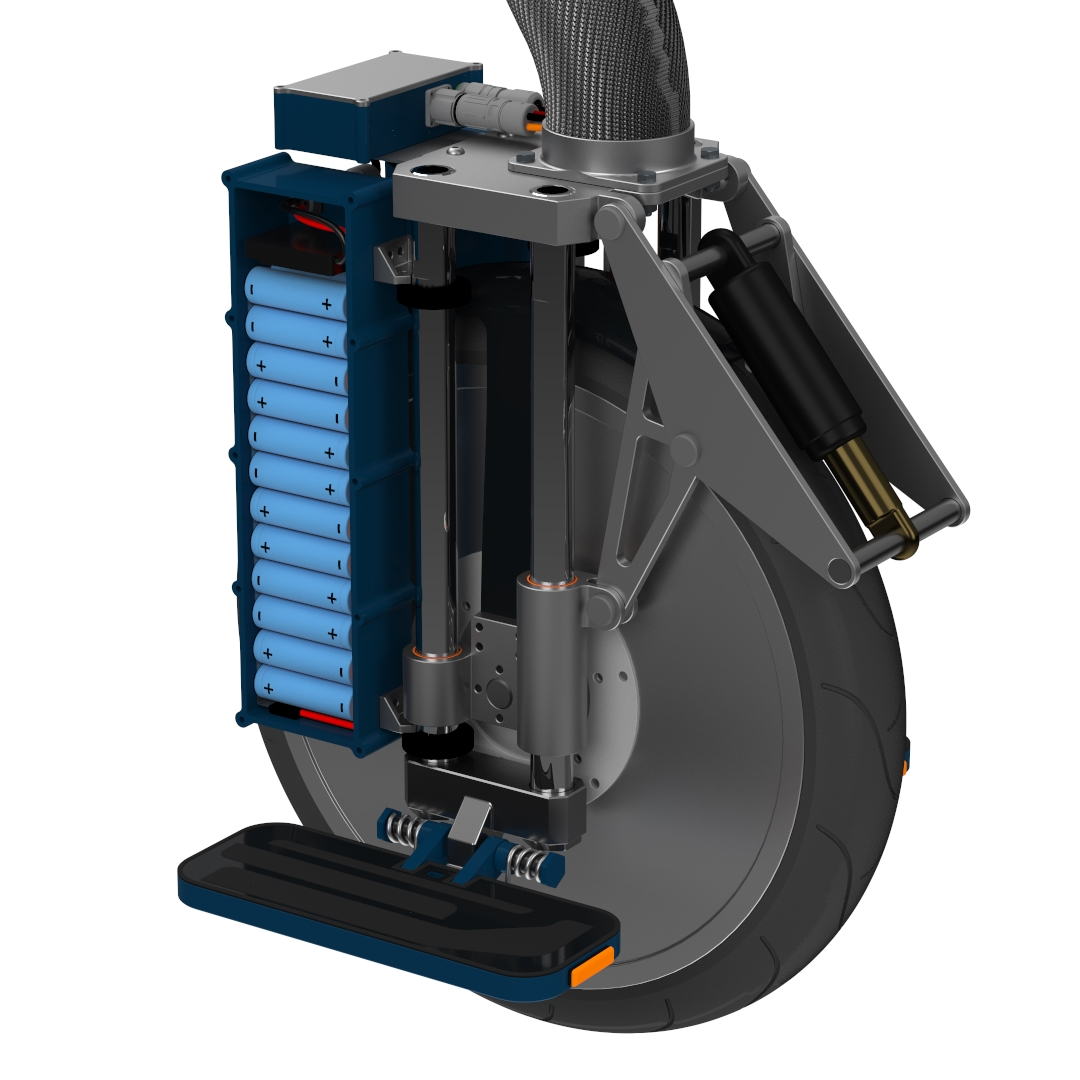
\includegraphics[height=120pt]{img/Rimac/1.jpg}
                \hspace{2cm}
                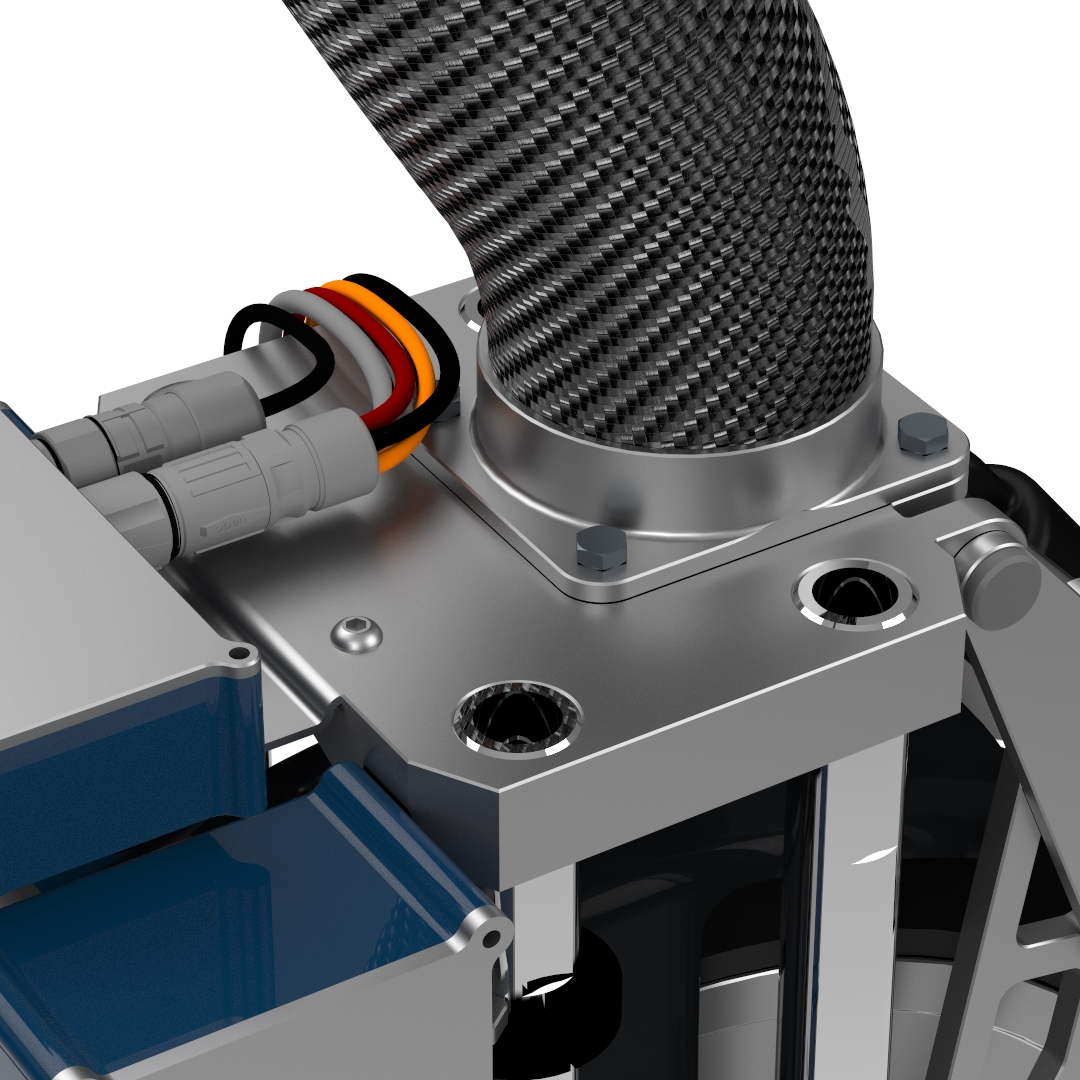
\includegraphics[height=120pt]{img/Rimac/2.jpg}
            \end{center}
            \vspace{5pt}
            Idealize and Design a Personal Transportation Vehicle (Sidewalk vehicle).\\
            Team-based project with students from 4 top European universities, featuring feedback sessions after each hackathon by company engineers. Selected as winning team.\\
            \begin{cvitems}
                \item {Hackathon 1: visions, user personas and functions \& requirements}
                \item {Hackathon 2: functional decomposition, morphological matrix and concepts development}
                \item {Hackathon 3: CAD design, FEM simulations, FMEA and cost analysis.}
            \end{cvitems}
            \vspace{4mm}
            \vspace{5pt}
        \end{minipage}
        \hfill
        \begin{minipage}{0.25\textwidth}
            \vspace{5pt}
            \begin{center}
                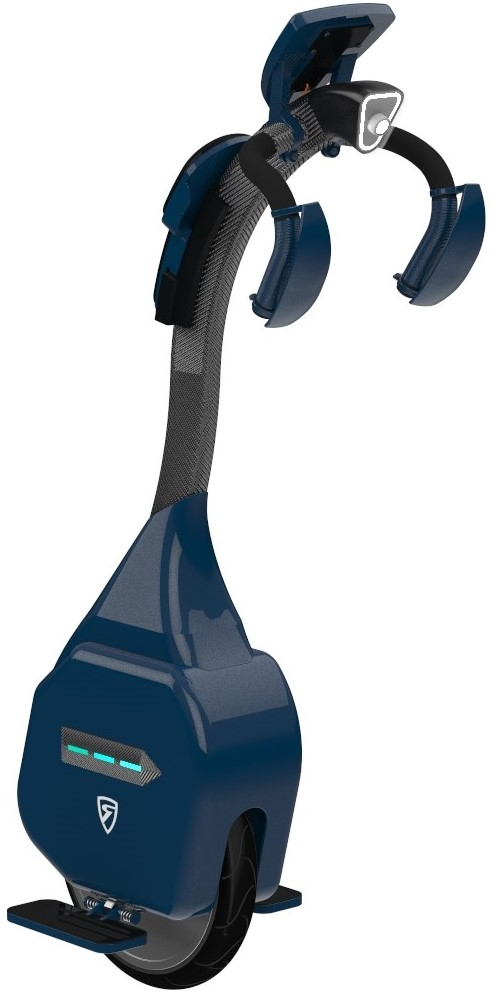
\includegraphics[height=200pt]{img/Rimac/3.jpg}
            \end{center}
            \vspace{5pt}
        \end{minipage}
    }
    %---------------------------------------------------------

    %---------------------------------------------------------
    \cventry
    {Done for fun or for my peer students} % Project name
    {Selection of other minor projects} % Institution
    {Personal Workshop, Como, Italy} % Location
    {2021 - PRESENT} % Date(s)
    {
        \begin{minipage}{0.45\textwidth}
            \vspace{5pt}
            \begin{center}
                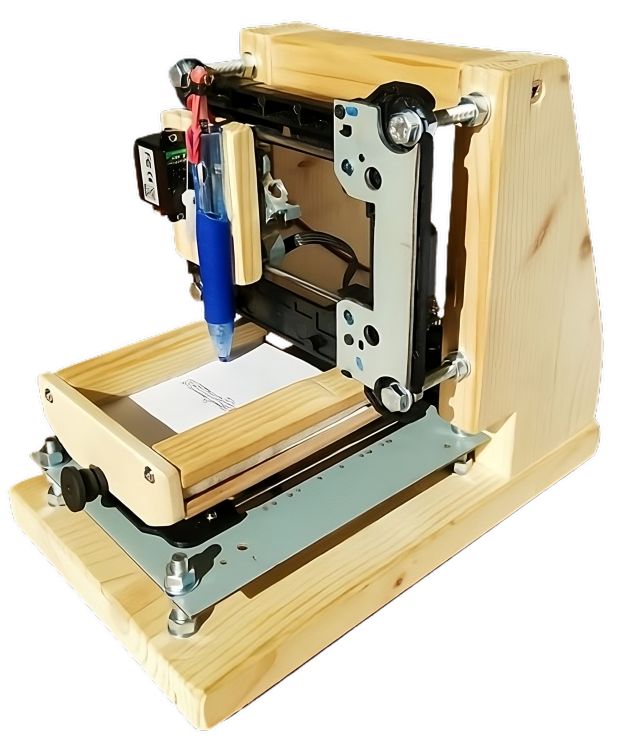
\includegraphics[height=150pt]{img/Minors/Gorlu.png}
                \hspace{4cm}
            \end{center}
            \vspace{5pt}
            CNC plotter to go from any digital image to its physical representation.\\
            \begin{cvitems}
                \item {Arduino based plotter with custom software.}
                \item {Canny edge detection algorithm.}
                \item {Recycled components from old DVD drives and wood.}
            \end{cvitems}
            \vspace{4mm}
            \vspace{5pt}
        \end{minipage}
        \hfill
        \begin{minipage}{0.45\textwidth}
            \vspace{5pt}
            \begin{center}
                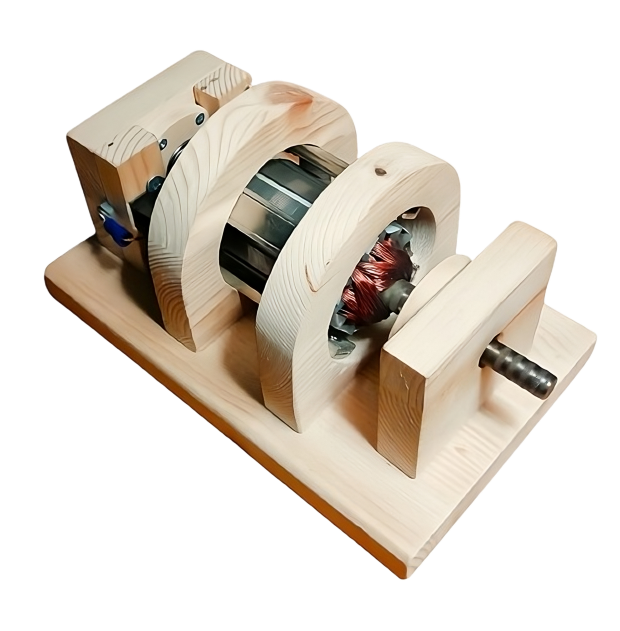
\includegraphics[height=150pt]{img/Minors/Joppo.png}
                \hspace{4cm}
            \end{center}
            \vspace{5pt}
            DC electric motor model to explain its working principle to my peer students.\\
            \begin{cvitems}
                \item {Recycled components from an old lawn mower and wood.}
                \item {Controllable in speed via a custom electrical circuit (diodes bridge and potentiometer).}
            \end{cvitems}
            \vspace{4mm}
            \vspace{5pt}
        \end{minipage}
    }
    %---------------------------------------------------------

\end{cventries}
